\documentclass{article}
\usepackage[utf8]{inputenc}
\usepackage{graphicx}
\usepackage{fullpage} % Makes full page size

%\bibliography{bibliography.bib}
\usepackage[authoryear,sectionbib,sort]{natbib}
\bibliographystyle{ecology_letters}

\title{Epigenetic simulation manuscript}
\author{Holly V. Moeller and the E5 Rules of Life Team }
\date{}

\begin{document}

\maketitle

\section*{NOTES TO COAUTHORS: Paper framework - 6 Sept 2024}


\noindent \textbf{BIBLIOGRAPHY DETAILS AND MINI TUTORIAL:}

We're using the ``natbib'' bibliography package. To insert an in-text citation use the ``citet'' command, e.g.: ``However, \citet{liew2018epigenome} found that ABC causes XYZ.'' For a parenthetical citation, use the ``citep'' command, e.g.: ''We know XYZ \citep{liew2018epigenome}.''

If you want to be fancier, you can also insert things into the citation parentheses before and after the citation using square brackets. For example, one might write: ''We know ABC \citep[see, e.g.,][]{liew2018epigenome}.''

\ 




\noindent \textbf{TARGET JOURNAL: Ecology Letters ``review and synthesis''}   

The goal of this paper is to use a simple epigenetic simulation as a framework to (1) synthesize the current state of understanding about the role of epigenetics in environmental matching, and (2) identify open questions in epigenetics research that should be prioritized. 

After describing the model, the paper is organized into three sections, each of which presents a core model prediction. Following presentation of the model's prediction, the section reviews empirical evidence and identifies open avenues of research. At the moment, the empirical review is classified into two categories: ``Correlational'' evidence and ``Mechanistic'' evidence.

I currently need help with:
\begin{itemize}
    \item Reading the manuscript for clarity, and especially responding to bold-faced queries in the text
    \item Writing text in the empirical section. There are many locations labeled in all caps where CITATIONS or writing from NAMED INDIVIDUALS are needed!
    \item Writing the introduction (currently in outline form)
    \item Brainstorming ideas for the conclusion
\end{itemize}


\clearpage

\section*{Introduction}

Organisms must maintain homeostasis in the face of environmental change -- \textbf{Should we narrow the focus here to marine invertebrates?}

Epigenetics is one mechanism by which they may respond to persistent environmental changes

Definition of epigenetics \& examples of it

We need to understand how epigenetic modifications are triggered, but our mechanistic understanding is poor

Mathematical frameworks can generate testable predictions about environmental triggers and mechanisms


We use our mathematical model to draw broad conclusions about the information organisms need to track their environments, and the types of environments that can be epigenetically tracked. We link these model predictions with hypotheses about the mechanisms, function, and distribution of epigenetic environmental tracking, and briefly survey the existing literature to identify correlational (i.e., evidence consistent with our model's hypotheses) and mechanistic (i.e., evidence supporting an explanatory linkage) existing information and knowledge gaps.


\section*{The Model}
To identify the circumstances under which an organism can track its environment using epigenetic changes, we developed a simple simulation model that represents the iterative process of adding and removing epigenetic markers to an organism's genome. These markers could represent changes in methylation state, histone modifications, or other mechanisms leading to up- or down-regulation of gene expression \cite{eirin2019marine}. Depending upon environmental conditions, certain gene expression strategies may be more favorable than others; an organism that adjusts its epigenetic state to enable such favorable expression patterns will therefore be better matched to its environment. Thus, organisms that are poorly matched to their environment should experience physiological benefits if they change their epigenetic markers to improve their match to the environment.

Here, we mimic this phenomenon by assuming that an organism experiences ``stress'' that is proportional to its phenotypic mismatch with local environmental conditions. The more stress an organism experiences, the greater the rate at which it remodels its epigenetic state. We first explore the epigenetic modification strategies that allow organisms to track their environments, and then mimic natural selection (by linking stress to fitness and assuming that the organisms with the highest stress levels are most likely to die and that those with the lowest stress levels are most likely to reproduce) to find optimal (i.e., stress-minimizing) epigenetic modification strategies.

\subsection{Model Components}


\noindent \textit{Defining the Environmental and  Epigenetic States}: We represent the states of both the environment and the organism as a binary string of sites that are either 1s or 0s, $\vec{E}$ (Figure \ref{fig:modeldiag}). Each of the $n$ positions in the string is a site that represents a hypothetical location in an organism's genome that could take on one of two epigenetic state values in response to environmental conditions. The environmental string's value at a particular position $E_i$ represents the organismal epigenetic state that would be best matched to the environment. %There are many possible interpretations of a single position on this string, which could represent a specific cytosine which should be methylated (=1) or demethylated (=0), or a gene or suite of genes corresponding to a particular phenotype that should be expressed (=1) or not expressed (=0) in order to best match the environment. 
A value of $1$ indicates that an organism with a stress-minimizing epigenetic state \textit{has} a marker in this location, and a $0$ indicates that stress-minimization is achieved by the \textit{absence} of an epigenetic marker. Note that there are many possible interpretations of a single position on this string, which could represent, e.g., a specific cytosine which should be methylated (e.g., CITE), or a gene or suite of genes whose expression is controlled by a cluster of epigenetic modifications made in concert \cite{adrian2020understanding}. We consider this string of epigenetic positions to represent the suite of an organism's genes that can be environmentally responsive; That is, we are neglecting genes that are silent or constitutively expressed, or that have invariant epigenetic states.

The environment can vary. There are various ways of implementing environmental change (i.e., shifts of $E_i$ from $0$ to $1$ or vice versa). We consider two possibilities: In one case, we periodically re-draw the entire environmental string, which represents an ``extreme event'' with an abrupt and random perturbation. In the second case, we allow the environment to vary cyclically by gradually shifting the environmental epigenetic state over time in a systematic manner. In the latter case, we can control both the speed (frequency of shifts) and magnitude (number of changed sites) of environmental change, allowing us to mimic cyclic perturbations like seasonality, interannual variation, and decadal cycles.
%(Other possibilities include: partial re-drawing, or a cyclic change representing seasonality.) Generally, environmental change is rare  compared to organismal epigenetic change, although environmental changes are large in magnitude when they occur (representing ``extreme events'').

\ 


\noindent \textit{The Organisms:} We use an individual based model to represent the population of living organisms in our model. Each individual is represented by its own binary string, $\vec{O}_j$, of the same length as the environmental string. Each position on an organism's string corresponds to the same position in the environmental string; this allows an individual organism to experience variable degrees of ``stress'' depending on the number of sites that are mismatched with the environment. Organisms can modify their epigenetic state according to the mechanisms outlined below, and may experience birth-death processes (with or without mutational change), depending upon the model formulation that is used. %Again, there are various interpretations of an ``organism'' in this model. For example, we could also think of each string as representing the nuclear genome of a single cell in a multicellular organism, or as representing the median state of an entire organism. \textbf{(NOTE: The assumption of a binary (either 0 or 1) state might lend itself more to the interpretation of a single cell.)}

\ 

\noindent \textit{Stress-Dependent Epigenetic Change:} We assume that organisms accelerate epigenetic remodeling when confronted with detectable physiological stress, which we here assume stems from a mismatch with their environment. We define stress as the average degree of mismatch with the environment across all $n$ possible epigenetic sites. Individual $j$'s level of stress $S_j$ is therefore given by:
\begin{equation}
   S_j = \frac{\sum_i ^n | E_i - O_{j,i} |}{n} .
\end{equation}
Note that this approach assigns each epigenetic location equal weighting, and assumes that incorrectly marked sites (i.e., organism = 1, environment = 0) and incorrectly unmarked sites (i.e., organism = 0, environment = 1) are equivalently stressful.

We assume that an organism makes epigenetic modifications proportional to the level of stress it is experiencing. In other words, if an organism is well-matched to its environment, its stress levels are low, and it will make few, if any, epigenetic changes. But when an organism's stress levels are high, it will accelerate rates of epigenetic remodeling in an attempt to more quickly achieve environmental optimality. Therefore, we represent each organism's probability of adding an epigenetic marker to a single site (i.e., changing that site's epigenetic state from a 0 to a 1, such as via methylation) within a round of epigenetic modification as proportional to its current stress level $S_j$, scaled by an individual-specific marker addition tendency $m_j$:
\begin{equation}
    M(j,t) = \min\left[m_jS_j(t),1\right].
\end{equation}
This stress-dependent probability is used to determine whether or not a currently unmarked site is marked during a given round of epigenetic change. Specifically, for each unmarked site, the algorithm draws a value between 0 and 1 from a uniform distribution. If this value is greater than the marking probability $M(j,t)$, an epigenetic marker is added. Per-round probabilities are capped at 1. Statistically, this means that the total number of sites that are marked in a given is drawn from a binomial distribution with a probability $M(j,t)$ and a number of trials equal to the number of presently demethylated sites (state = 0). 

The removal of markers is scaled similarly, with an individual marker deletion tendency $d_j$:
\begin{equation}
    D(j,t) = \min \left[d_jS_j(t),1 \right].
\end{equation}

Addition and deletion probabilities tell us how likely an organism is to remodel each position in its string $\vec{O}_j$ at each timestep. However, these probabilities may change if the organism has information about which sites are currently mis-matched with its environment. Such environmental information might be collected when, for example, excess gene products inhibit gene expression. %When environmental conditions halt the use of these gene products, the gene is then occluded, and epigenetic markers can be removed. \textbf{(-- NB: Need help here to think of a good example for why feedback is in marker removal!)} 
We use a scalar to increase the probability of ``correct'' epigenetic changes. Thus, the probability of \textit{preferentially} removing an epigenetic marker from a mismatched site (i.e., a location where the environmental state is 0 and the organismal state is 1) is given by:
\begin{equation}
    D_p(j,t) = \min\left[(p_j+d_j)S_j(t),1\right].
\end{equation}
where $p_j$ is the individual-specific preferential removal tendency. Although both addition and removal can occur preferentially, here we consider only preferential removal. \textbf{(NB: Made this choice to get ``spikes'' in demethylation after an environmental change. Maybe consider the alternate case in a supplement?)}

Because similar cellular equipment is likely used for both preferential and baseline removal of epigenetic markers, we assume that these two probabilities must be related to one another. For example: if an organism has produced a lot of cellular enzymes that demethylate cytosines, then these enzymes will likely increase both preferential (i.e., environment-informed; $p_j$) and random ($d_j$) marker removal tendencies. We therefore assume that there is an overall removal tendency $o_j$, that is governed by the production of such machinery, and that an environmental information parameter, $\epsilon$, links the random and preferential change tendencies, which are centered around this overall tendency:
\begin{equation}
    o_j = \frac{ d_j\left( 1 - \epsilon \right) + p_j \left( 1+ \epsilon \right) }{2}.
\end{equation}
Here, we choose $0 \leq \epsilon \leq 1$ so that all removal probabilities are nonnegative.

It is convenient to link the addition and removal of epigenetic markers, which we do with the parameter $b$, that scales the tendency of removal relative to the tendency of addition:
\begin{equation}
    m_j = b o_j = \frac{b\left[ d_j\left( 1 - \epsilon \right) + p_j \left( 1+ \epsilon \right) \right]}{2}.
\end{equation}
If $b > 1$, marker removal is more stress-sensitive than marker addition, and if $b < 1$, the opposite is true.

In most of our simulations, we focus on an environment that has roughly equal numbers of marked and unmarked sites. That is, the proportion of epigenetic sites in state $1$ is approximately $0.5$. Thus, an organism whose genome is wholly marked and an organism whose genome is wholly unmarked both experience high stress levels of $0.5$, which is also the mean expected stress level of an organism with an entirely random epigenetic strategy. %\textbf{(This paragraph kind of feels like it belongs in the ``environment'' description, but I needed to define stress first, which only shows up in the organism section...)}

\ 




\noindent \textit{Evolutionary algorithm:} To efficiently determine the optimal epigenetic modification strategy, we employed a pseudo-evolutionary algorithm. This algorithm incorporates birth-death processes (which occur once every XXXXX epigenetic remodeling steps) and mutation (which occurs less frequently, once every XXXXX epigenetic remodeling steps), and allows the population of individuals to ``find'' stress-minimizing combinations of epigenetic marker addition and removal tendencies.

For birth-death processes, we assume that natural selection acts on the population, such that when a birth-death event occurs, organisms that are presently experiencing the highest levels of stress are the most likely to die. Meanwhile, organisms with the lowest stress levels are most likely to reproduce. Our current algorithm assumes strong natural selection, such that the organism with the highest stress is eliminated (= death event), and the organism with the lowest stress is duplicated (= birth event). Birth events duplicate an organism's parameters (e.g., $m_j$ and $d_j$) as well as its present epigenetic state $\vec{O}_j$.

Mutational events can impact an organism's tendency for the addition or removal of epigenetic markers. When a mutation event happens, we draw a new tendency from a normal distribution centered around the organism's present tendency. Tendencies are constrained to be non-negative; thus a mutation that results in $m_j<0$ or $d_j<0$ will be rounded to $m_j=0$ or $d_j=0$, respectively.


\subsection{Algorithm Steps}
In our model, at each time step, events occur in the following order, for each individual:
\begin{enumerate}
    \item The individual's stress is computed.
    \item Epigenetic marker addition (changes from 0 to 1) occurs.
    %\item Stress is re-computed. \textbf{NOTE: Results don't really change if I skip this step, or if I swap order of methylation and demethylation. Let's talk about what choices are best?}
    \item Epigenetic marker removal (changes from 1 to 0) occurs.
\end{enumerate}

Following these individual events, population-level events occur in the following order. Note that not all events take place at every time step:
\begin{enumerate}
  \setcounter{enumi}{4}
    \item A single birth-death event, if any, occurs.
    \item A single mutation event, if any, occurs.
    \item Environmental change, if any, occurs.
\end{enumerate}

\textit{A note on timescales:} In our model, events occur with different frequencies. In order from most frequent to last, we have:
\begin{enumerate}
    \item Changes to an organism's epigenetic state. These occur every timestep, although the rate at which they occur depends upon an organism's tendency for marker addition and removal.

    \item Mutational change and birth-death processes. These occur less frequently than epigenetic changes, but more frequently than environmental shifts. We generally assume that birth-death events are more frequent than mutations, so that the fitness effects of a mutation can play out for several generations.

    \item Environmental change. Shifts in the environment are relatively rare, and occur about once every 100 epigenetic timesteps. 
\end{enumerate}

The frequency of each of these events implies an interpretation of the model's timescale. For example, the frequency of epigenetic change with respect to generation time implies that we are modeling within-generation epigenetic change, rather than epigenetic remodeling that occurs only during reproduction.


\begin{figure}
    \centering
    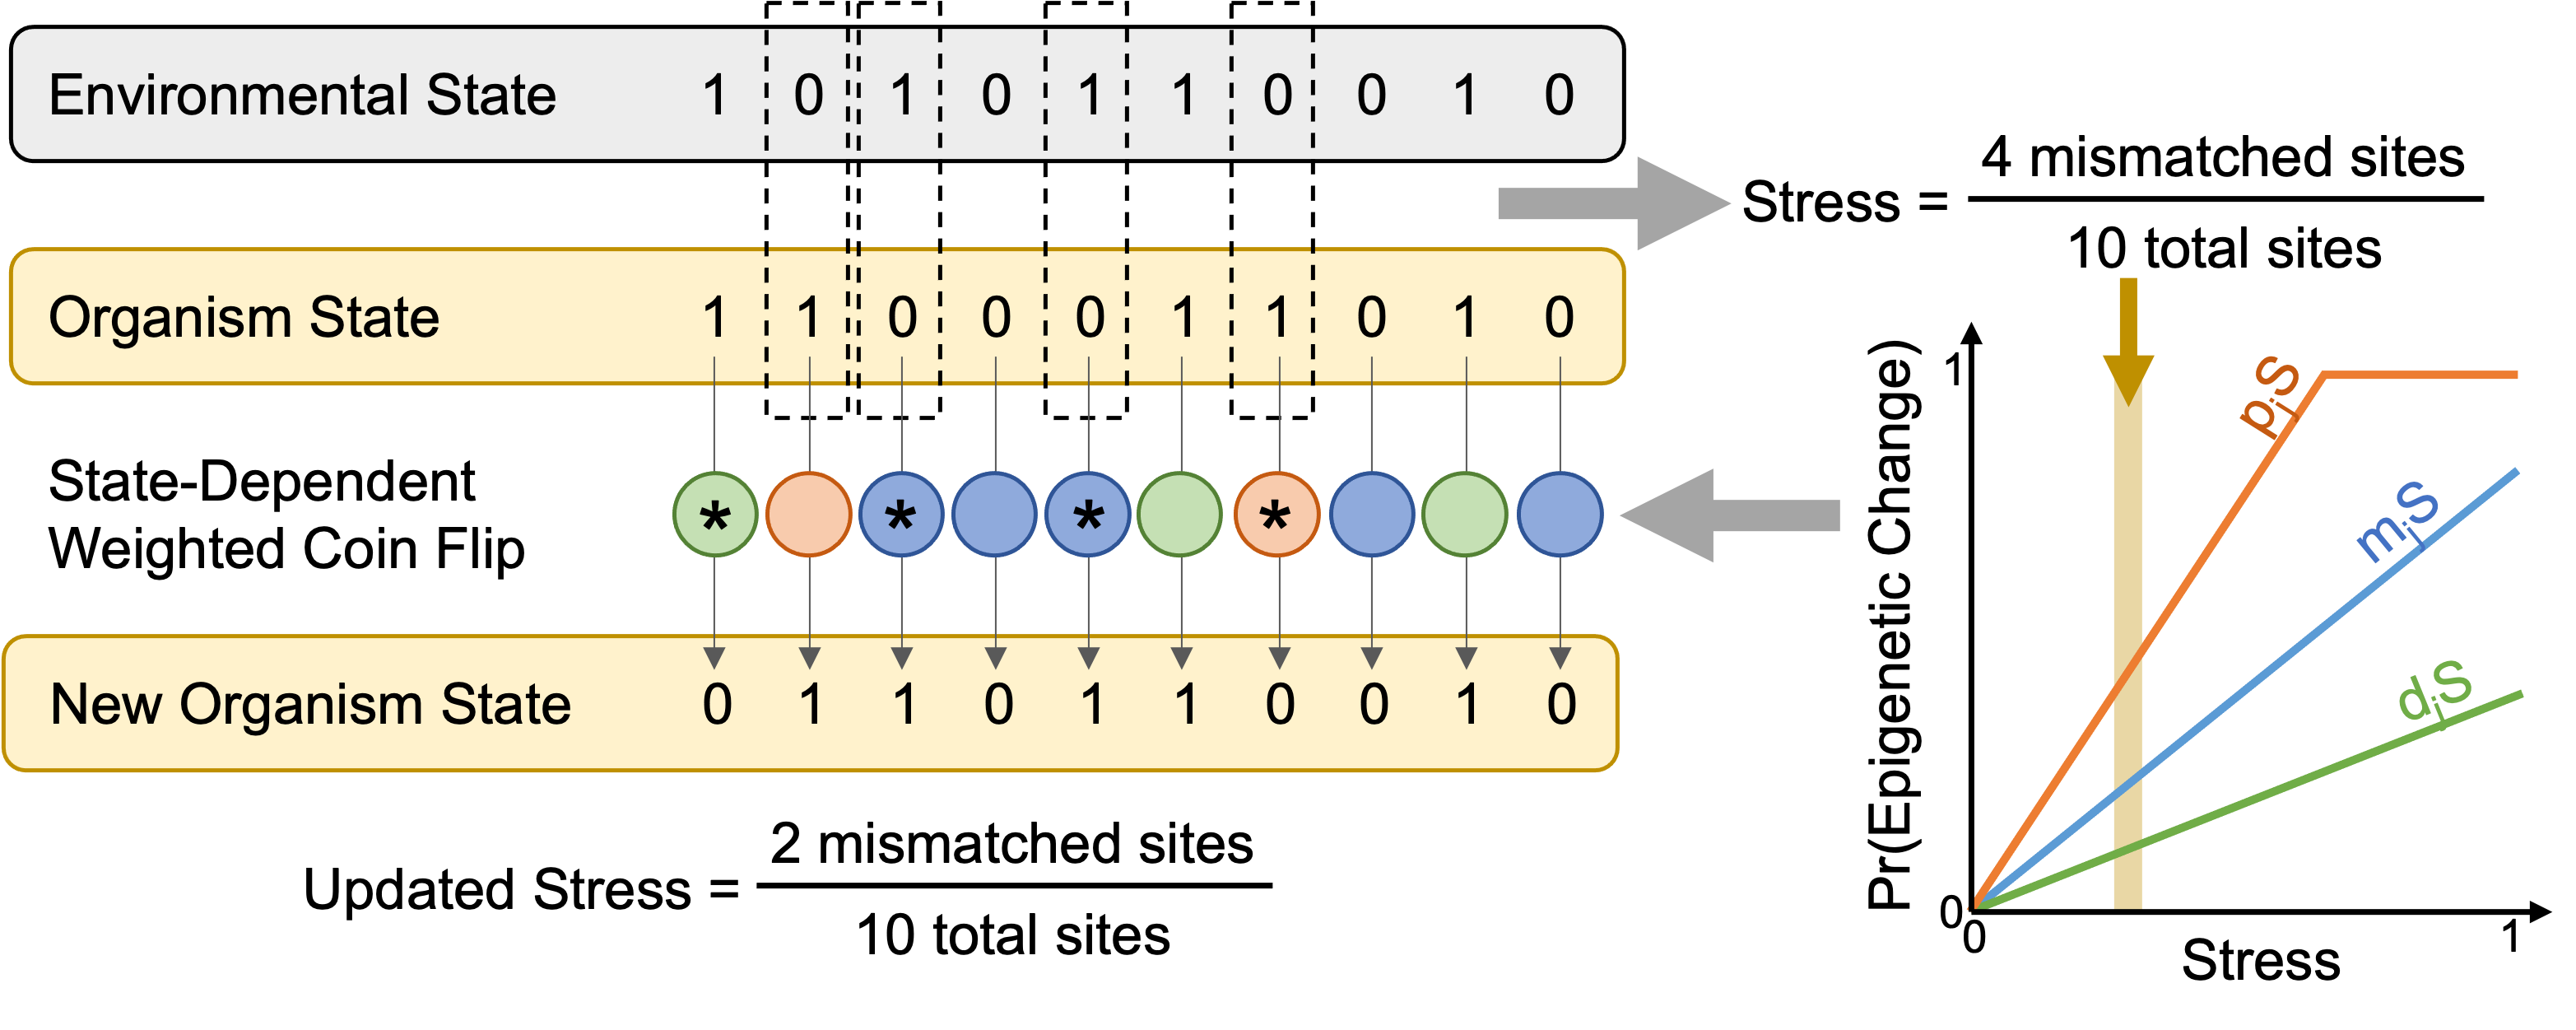
\includegraphics[width=\textwidth]{Figures/ModelDiag_v1.png}
    \caption{Conceptual diagram showing epigenetic modification. First, the organism's state is compared to the environment and stress is computed. Based on stress levels and epigenetic change tendencies, the probability of an epigenetic change is computed. These probabilities are used to weight ``coin flips'' that determine which specific locations in the genome undergo random addition of epigenetic markers (blue), random removal of markers (green), or preferential removal of markers (orange). In the diagram, coin flips that result in epigenetic change are marked with a star. Following these changes, the organism's stress can be recomputed (beginning the next timestep); in this case, stress has been reduced from 0.4 (4 mismatched sites) to 0.2.}
    \label{fig:modeldiag}
\end{figure}

\subsection{Model Analysis}
We used our model to address three questions about how epigenetic modifications could allow organisms to track their environment. We asked (1) whether organisms must receive some information about the state of the external environment in order to be able to track the environment; (2) what relative rates of addition and removal of epigenetic markers allow an organism to minimize its stress by tracking its environment; and (3) under which environmental conditions epigenetic change is an effective mechanism for environmental tracking. Below, we describe our analytical approach and the model's predictions for each query. We compare the model's predictions with existing empirical knowledge, and identify key research priorities to address any knowledge gaps.





\clearpage

\section{Results}

\subsection{Tracking the environment requires information}
How do organisms gather information about the environment around them, and is this information necessary for them to tune their epigenetic state to match environmental needs? While stress from environmental mismatch can be measured at the aggregate scale, it is less clear how organisms might identify which specific genes should be activated or deactivated based on environmental cues. Therefore, we first used our model to investigate what information organisms need to detect about their (mis)match to the environment in order to track the environment epigenetically.


The emperical evidence for this in marine invertebrates is limited however there are a handful of studies can be separated in two categories; acute assessments in epigenetic state upon environmental change and long-term assessments of epigenetic state in relation to environmental conditions. Much of the work looking at acute responses include work in molluscs and cnidarians. For mollusc particulary attention has been given to changes in response to ocean acidificaiton. Shifts in DNA methylation landscapes have be found in response to ocean acidification in the Crassostrea viginica in mantle \cite{10.3389/fmars.2020.566419} and gonad \cite{0.3389/fmars.2020.00225} the mantle \cite{10.1111/gcb.15675} and larvae \cite{10.1016/j.marenvres.2020.105217, 10.1111/mec.16751} of Crassostrea hongkongensis, and the reproductive tissue \cite{10.1186/s12864-022-08781-5} of female Crassostrea gigas. These shifts are as might be expected associated with different gene sets depending on the tissue. Variability can be seen across sex to as in a recent study where fter a 30-day exposure to control (572 ppm) or elevated pCO2 (2,827 ppm) condtions, whole genome bisulfite sequencing revealed 89 differentially methylated loci in females and 2,916 differentially methylated loci males (2,916) \cite{10.1101/2024.04.04.588108}. In cnidarians, the response to ocean acidification has been less studied but a recent study in the coral Acropora millepora found that the response to ocean acidification



\subsubsection{Model Results: The mathematical model predicts information-dependent tracking.}
We examined the ability of an organism to track a stochastically changing environment as a function of its degree of information about the state of that environment. Specifically, we varied the magnitude of the difference between preferential and random marker removal probabilities as a proxy for the amount of information an organism has about its environment. When no information is present, all changes to epigenetic state occur stochastically, such that $\epsilon = 0$ and $d_j = p_j = m_j$. When all marker removal is information-based, the only sites chosen for removal are those that produce matches to the environment. In this case, $\epsilon = 1$, such that $d_j = 0$ and $p_j = 2m_j$. 

We found that %, in the absence of birth-death processes that vertically transmit preferable epigenetic states via natural selection, 
only organisms that can obtain environmental information are able to track the environment (Figure \ref{fig:envfeedback}). These organisms experience transient increases in stress when the environment changes, triggering a period of marker removal (Figure \ref{fig:envfeedback}b). Over time following the environmental perturbation, these organisms adjust their epigenetic state to match their environment, returning their mean number of epigenetic markers to the pre-disturbance state and lowering their stress levels from $\approx 0.5$ (the mean expected proportion of mismatched sites when the environment and organism are drawn randomly) to values as low as 0.15 (a $15\%$ mismatch with their environment). 

The magnitude of stress reduction depends on how successfully organisms can decouple random ($d_j$) and preferential ($p_j$) marker removal (Figure \ref{fig:envfeedback}c). The optimal solution would be to set $d_j = 0$ so that no random marker removal occurs, and then to increase $p_j$ without bound so that the probability of accurately removing markers from mismatched sites is high, even when stress is low. However, it seems unlikely that an organism would be able to completely avoid inadvertent marker removal: First, marker removal is likely during cell division because epigenetic markers are not always copied over to new strands of DNA (CITATION). Second, when there is high production of epigenetic modification enzymes related to stress response (i.e., if $p_j$ is large), it seems reasonable to suppose that some inadvertent marker removal will also take place. Thus, in our subsequent analyses, we coupled these rates to each other by setting $\epsilon = 0.8$. %\textbf{I chose 0.8 for interesting dynamics, but probably need to talk about this w/ the empiricists.}


\begin{figure}
    \centering
    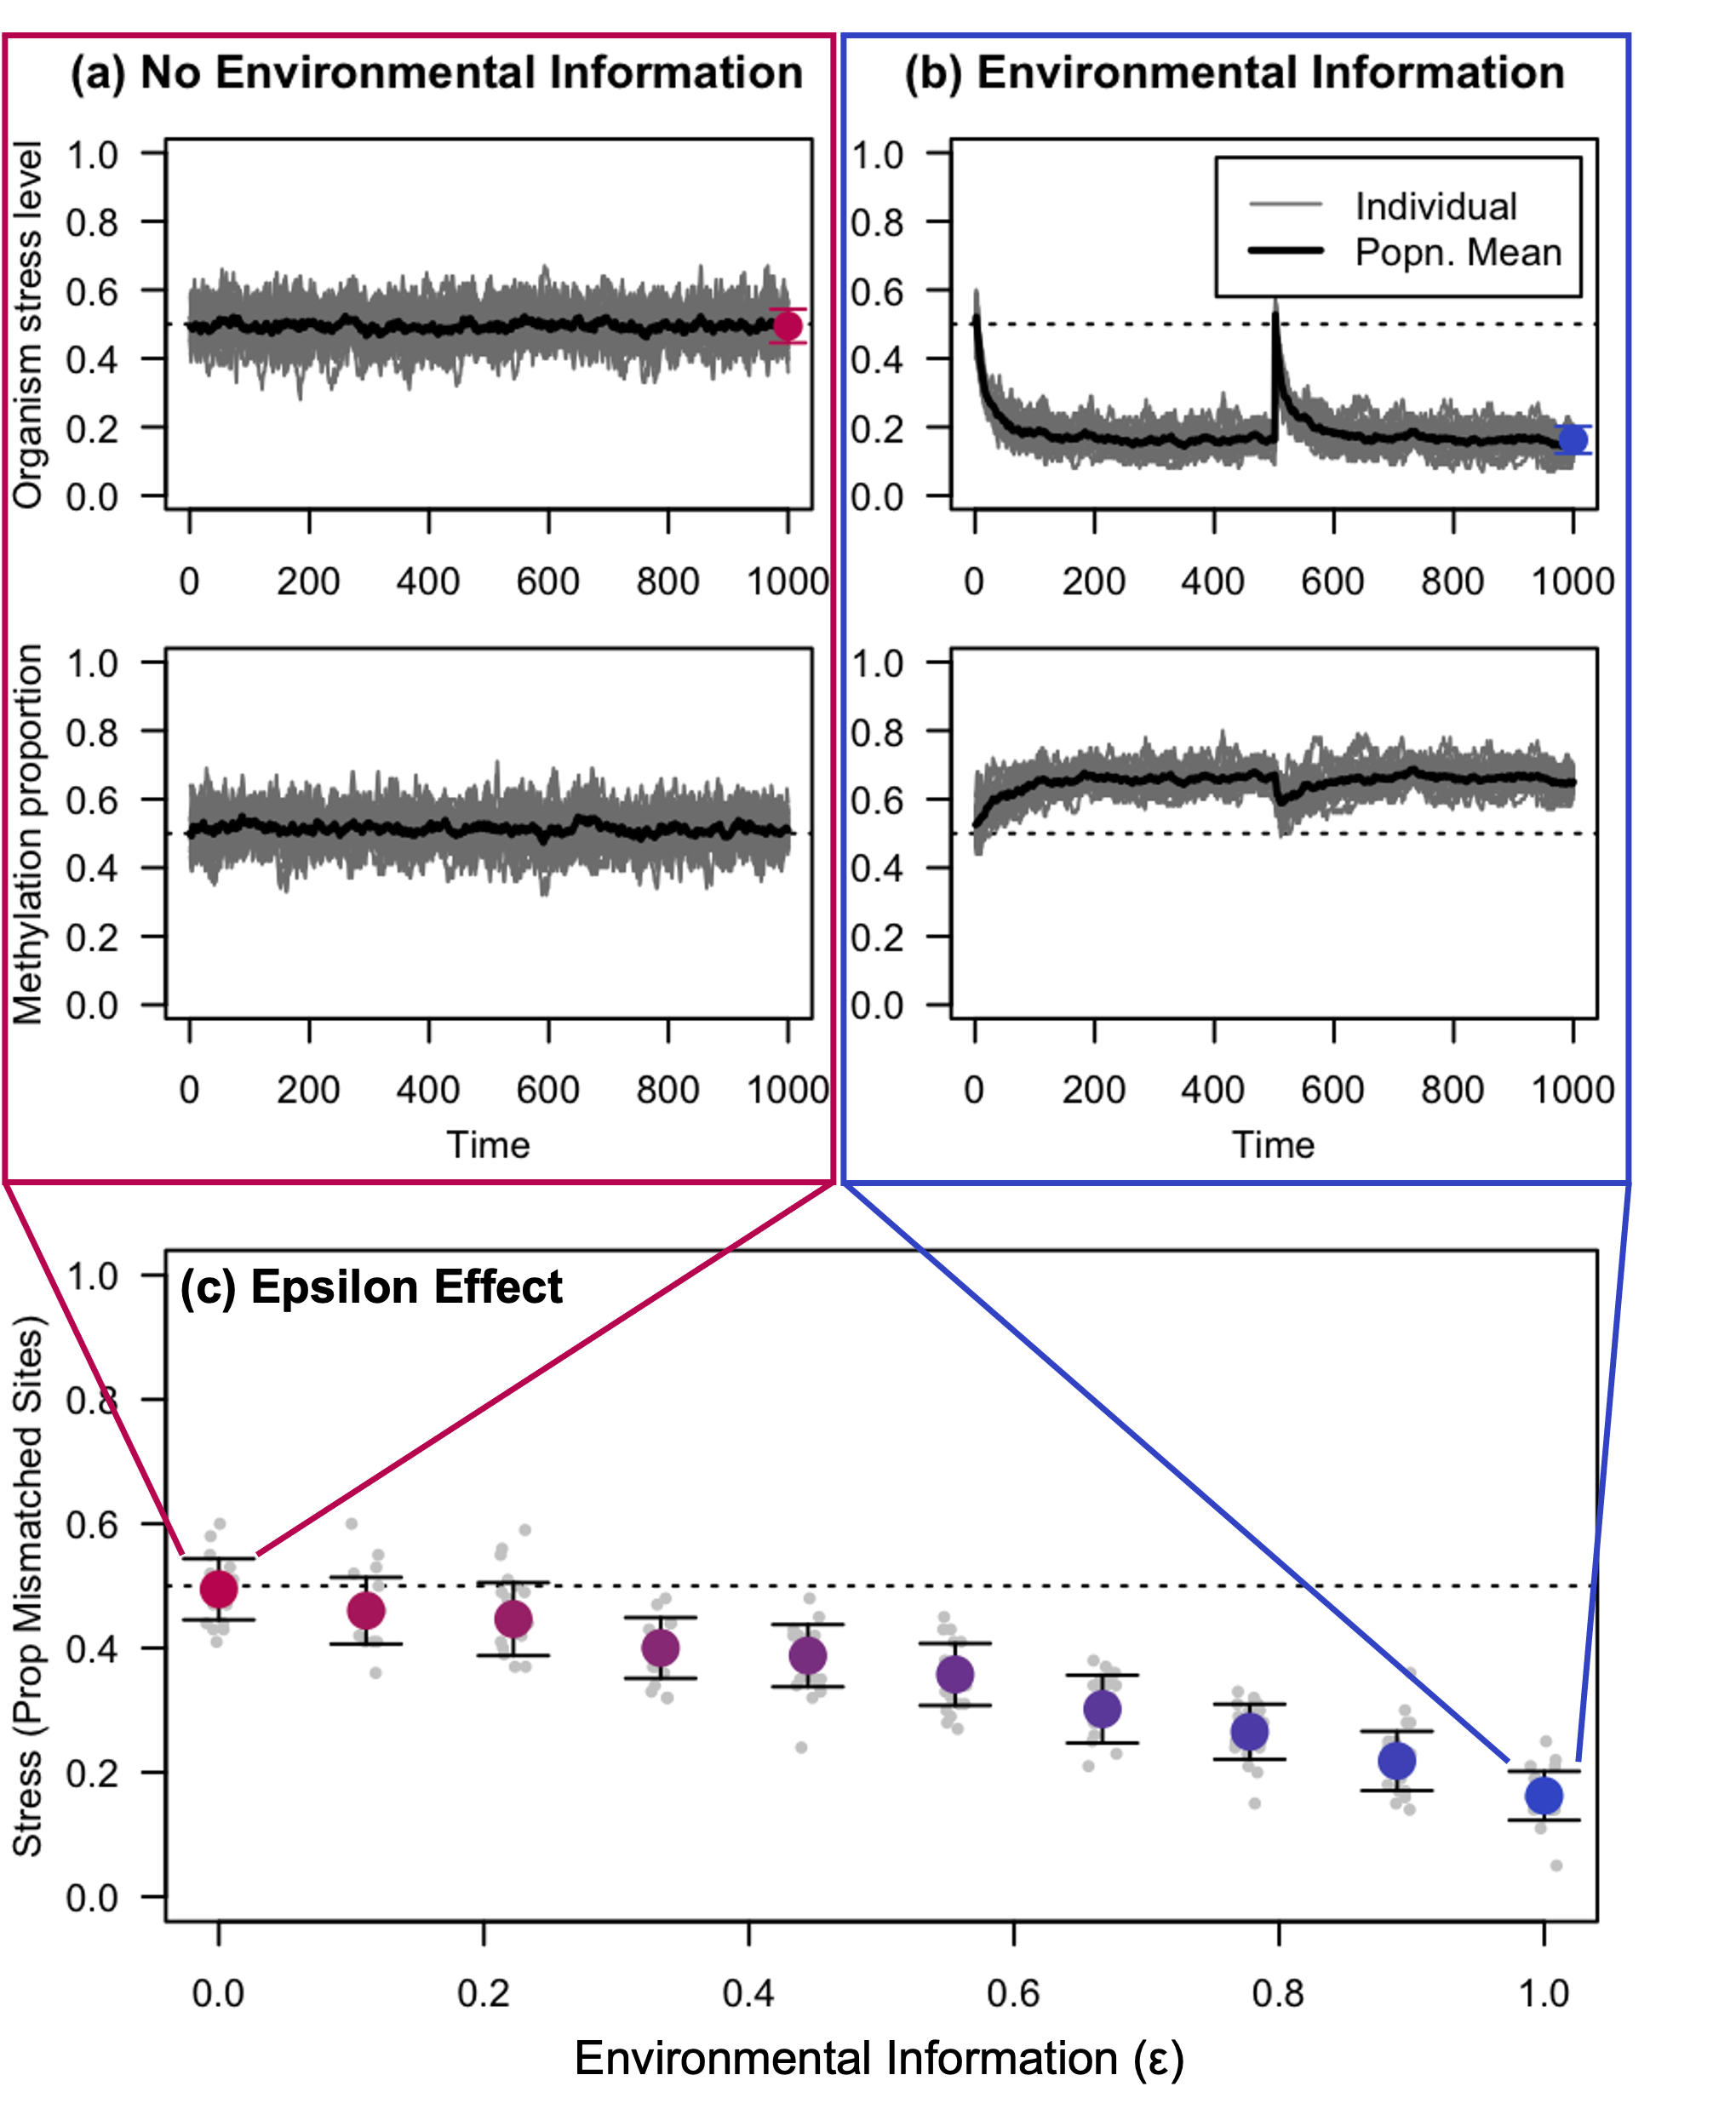
\includegraphics[width=.8\textwidth]{Figures/Fig_EnvironmentalFeedback_Consolidated.png}
    \caption{\textbf{Effects of environmental information on organismal stress.} Top: Timeseries showing a group of 20 organisms tracking (or failing to track) their environment over time. Without environmental information stress levels hover around the mean expectation of 0.5 (a), but with environmental information, the organisms are able to reduce their stress levels within about 100 timepoints (b). Bottom: The larger the difference in baseline and preferential marker removal tendencies, the better the organism's performance. Simulations are for 50 organisms with a baseline marker addition tendency of 0.2 tracking an environment with an epigenetic marker abundance of 0.5. Bars show standard deviation around the mean.}
    \label{fig:envfeedback}
\end{figure}

\subsubsection{Correlational Evidence: Empirical studies demonstrate repeated, directional epigenetic shifts.}

What empirical evidence exists that marine invertebrates use environmental information to directionally shift their epigenetic states in order to track the environment? Numerous studies have shown that organism phenotypes may vary predictably across gradients in environmental condition (CITATIONS) and may shift directionally in response to environmental perturbations like ABC (CITATIONS) and DEF (CITATIONS). A growing body of evidence is beginning to link these phenotypic changes to epigenetic changes.
For example X in oysters. The initial indication of inducible epigenetic change by DNA methylation in corals was documented in the enviornmentally sensitive P. acuta, but not the envioronmnetally more tolerant M. capitata \cite{putnam2016ocean}

\citet{liew2018epigenome}

For example TKTKTKTKTK (CITATIONS). 

In addition, experimental manipulations of organisms' environments have produced directional changes in epigenetic state. For example, TKTKTKTK and TKTKTKTK. Notably, studies that track bulk methylation have demonstrated transient pulses of demethylation (CITATIONS), consistent with our model's prediction of transient loss of epigenetic markers immediately following an environmental perturbation (Figure \ref{fig:envfeedback}C). EXAMPLE: Plants global reduction in methylation [[Steven can write something?]]


\subsubsection{Mechanistic Evidence: What mechanisms might allow organisms to translate environmental information into epigenetic modifications?}

Our model posits that these directional changes arise gradually, from the accumulation of a few directional (a.k.a. information-based) marker removals amidst a largely random set of additions and removals. In this way, our model mimics what we postulate to be the actual mechanism of epigenetic change, in which enzymes and substrates interact semi-randomly in the nucleus (CITATION). [[CHEMA TO WRITE MORE]]

However, consistent changes in phenotype, and changes in epigenotype, with environmental change suggest a mechanistic linkage between an organism's environment and its epigenetic state (e.g., that some epigenetic modifications occur non-randomly, as in our model). Yet the mechanisms by which organisms use environmental cues to modify gene expression networks remain unclear. Some mechanistic linkages do exist in in vertebrates. For example, in fish, changes in temperature can alter the methylation of the promoter region that controls expression of ABCDEFG gene, altering sex [[STEVEN TO WRITE/CHECK]]. 

In corals, a putative mechanism of epigenetic response to changes in ocean pH may involve physiological changes to the calcification process. [[HOLLIE TO WRITE/CHECK: proposed hypothesis: Change in pH triggers changes in physiology, followed by epigenetic changes in methylation \& histone modification. See: Liew et al OA 1-year: porosity of skeleton \& kinases – morphology \& cell size; histone modifications. [[Hollie to write]] Li et al  - ]]

Understanding the generality of these mechanisms requires first determining how different epigenetic markers (in different regions of the genome) act to alter gene expression. For example, while in vertebrates methylation is generally understood to INCREASE (CHECKCHECKCHECK) gene expression (CITATIONS), in invertebrates the directionality is less certain (CITATIONS) EXAMPLES TKTKTKTK. Thus, environmental changes that impact the activity of cellular machinery involved in the addition (or removal) of epigenetic markers may have differential impacts on specific gene networks.

Closing these knowledge gaps will require additional mechanistic studies linking environmental change to epigenetic state. Ideally, these studies should identify the types and timing of epigenetic changes triggered by known environmental changes. Collectively, identifying putative mechanistic pathways will allow us to understand the full scope of potential epigenetic alterations and, in turn, the magnitude and speed of environmental change that organisms may be able to withstand.

There is stochasticity in how these enzymes function, so some equipment for addition and removal must be present at all times

\clearpage

\subsection{``Optimal'' coupling of epigenetic change tendencies depends on the environment}

The dynamic process of adding and removing epigenetic markers allows for the location of these markers to shift over time, enabling an organism to respond to changes in its environment. However, in order to maintain epigenetic states, the loss and addition of these markers must be roughly balanced. Therefore, we next studied how marker addition and removal tendencies (which in our model underlie the linkage between an organism's stress and its rate of epigenetic change) must be coupled to one another in order to allow for epigenetic tracking.


\subsubsection{Model Results}

If marker addition and removal probabilities become too decoupled, an organism can lose all epigenetic markers (if $b >> 1$ such that $d_j, p_j >> m_j$) or add markers to all of its genome (if $b<<1$ such that $m_j >> d_j,p_j$). In an environment with an average marker abundance of $0.5$ (as studied here), an organism that has lost (or gained) all of its epigenetic markers experiences a high level of stress (0.5). Therefore, the more mismatched the marker alteration tendencies, the higher the stress level (Figure \ref{fig:methylmismatch}).

\begin{figure}
    \centering
    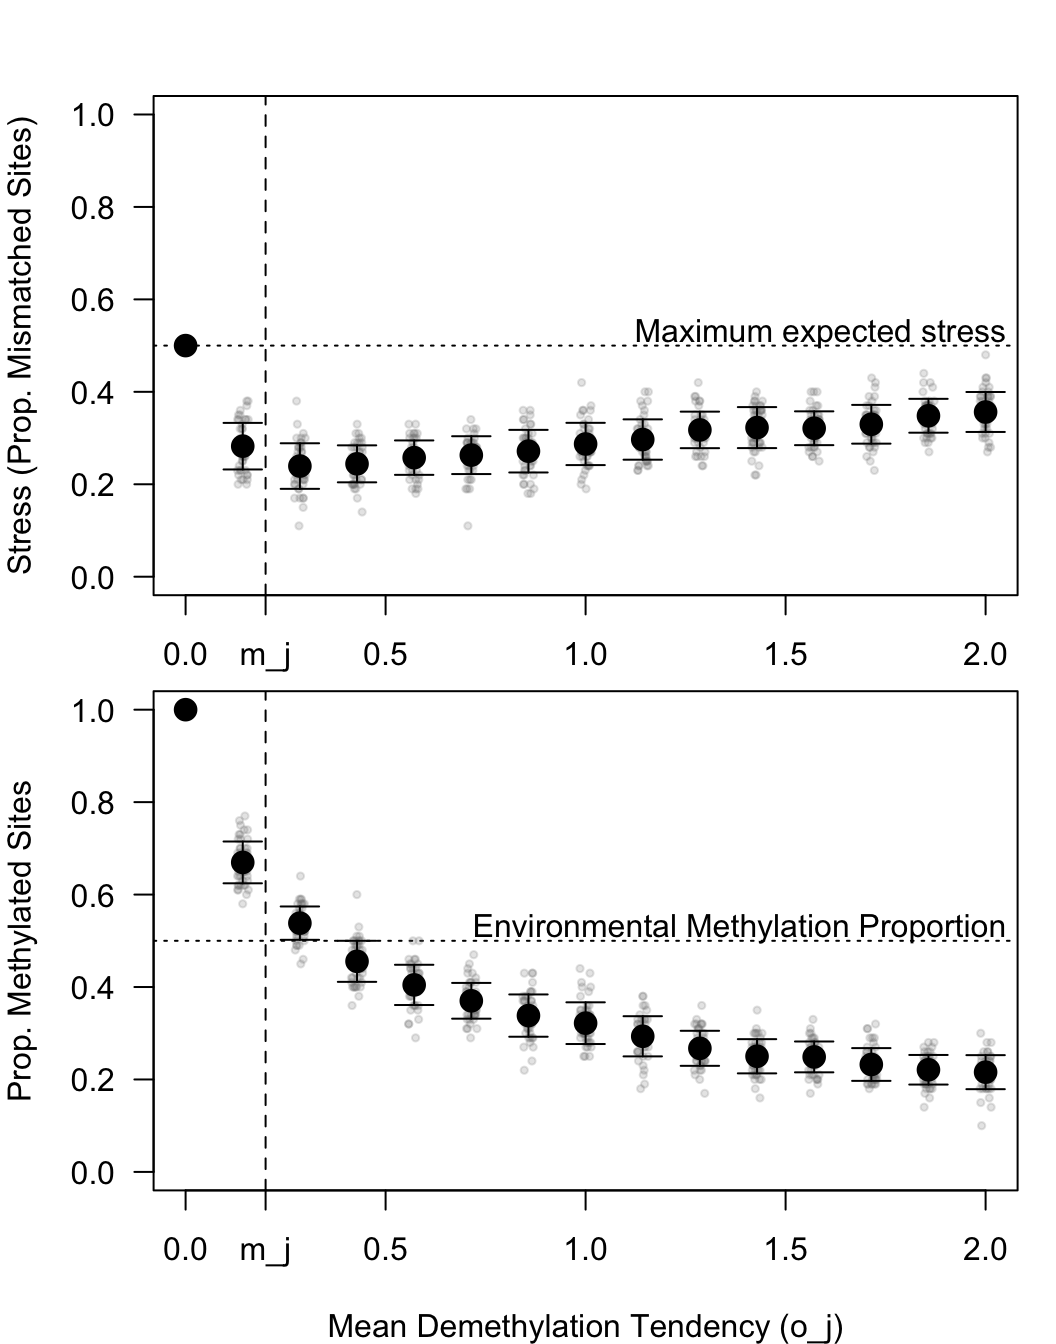
\includegraphics[width=0.8 \textwidth]{Figures/Fig_DemethDependence.png}
    \caption{\textbf{FOR SUPPLEMENT:} Dependence of stress and proportion sites with markers on marker removal tendency. Stress is minimized when mean marker removal tendency ($o_j$) is similar to marker addition tendency ($m_j$), resulting in the proportion of epigenetic markers on organism genomes slightly exceeding that required to match the environment (0.5). Simulations are for 50 organisms with a baseline marker addition tendency of 0.2 (vertical dashed line). Bars show standard deviation around the mean. The null expectation for stress and the proportion of environmental sites marked (0.5, dotted horizontal line) are also shown for reference. \textbf{HOLLY NEEDS TO ALTER FIGURE LABELS}}
    \label{fig:methylmismatch}
\end{figure}

We computed optimal pairs of marker addition and removal tendencies by fixing the former and using a pseudo-evolutionary algorithm to find values of the former that minimized organismal stress. Specifically, we modified our algorithm to include birth-death processes that eliminated the highest stress individual and replaced that individual with a duplicate of the lowest stress individual (mimicking reproduction of the highest fitness individual). Birth-death processes occurred every 10 rounds of epigenetic change, and every tenth birth-death event also involved a mutation in the marker removal tendency. When a mutation occurred, a new mean marker removal tendency was drawn from a normal distribution with standard deviation 0.1 centered around the parent's removal tendency. We bounded the distribution at zero, so that negative tendencies could not arise. Thus, over time, populations evolved marker removal tendencies that minimized stress (Figure \ref{Sfig:evolutionts}). %We repeated this pseudo-evolutionary approach for several rounds to confirm our findings.

Our results highlight the importance of coupling epigenetic marker regulatory tendencies. Generally, higher marker addition tendencies necessitate higher marker removal tendencies so that the average level of genome marking remains constant (Figure \ref{Fig:Evolution3panel}). Decoupling between these rates produces high stress either because of rampant marker removal (if $o_j > m_j$) or addition (if $o_j < m_j$) (Figure \ref{SFig:StressHeatmap}). However, the exact coupling of these tendencies depends upon environmental conditions. For example, when the environment has relatively few epigenetic markers, marker removal should outstrip addition to keep the organism's overall amount of epigenetic markings low (Figure \ref{Fig:Evolution3panel}a), but when the environment requires a high amount of epigenetic markers, organisms should evolve relatively low demethylation tendencies (Figure \ref{Fig:Evolution3panel}).


\begin{figure}
    \centering
    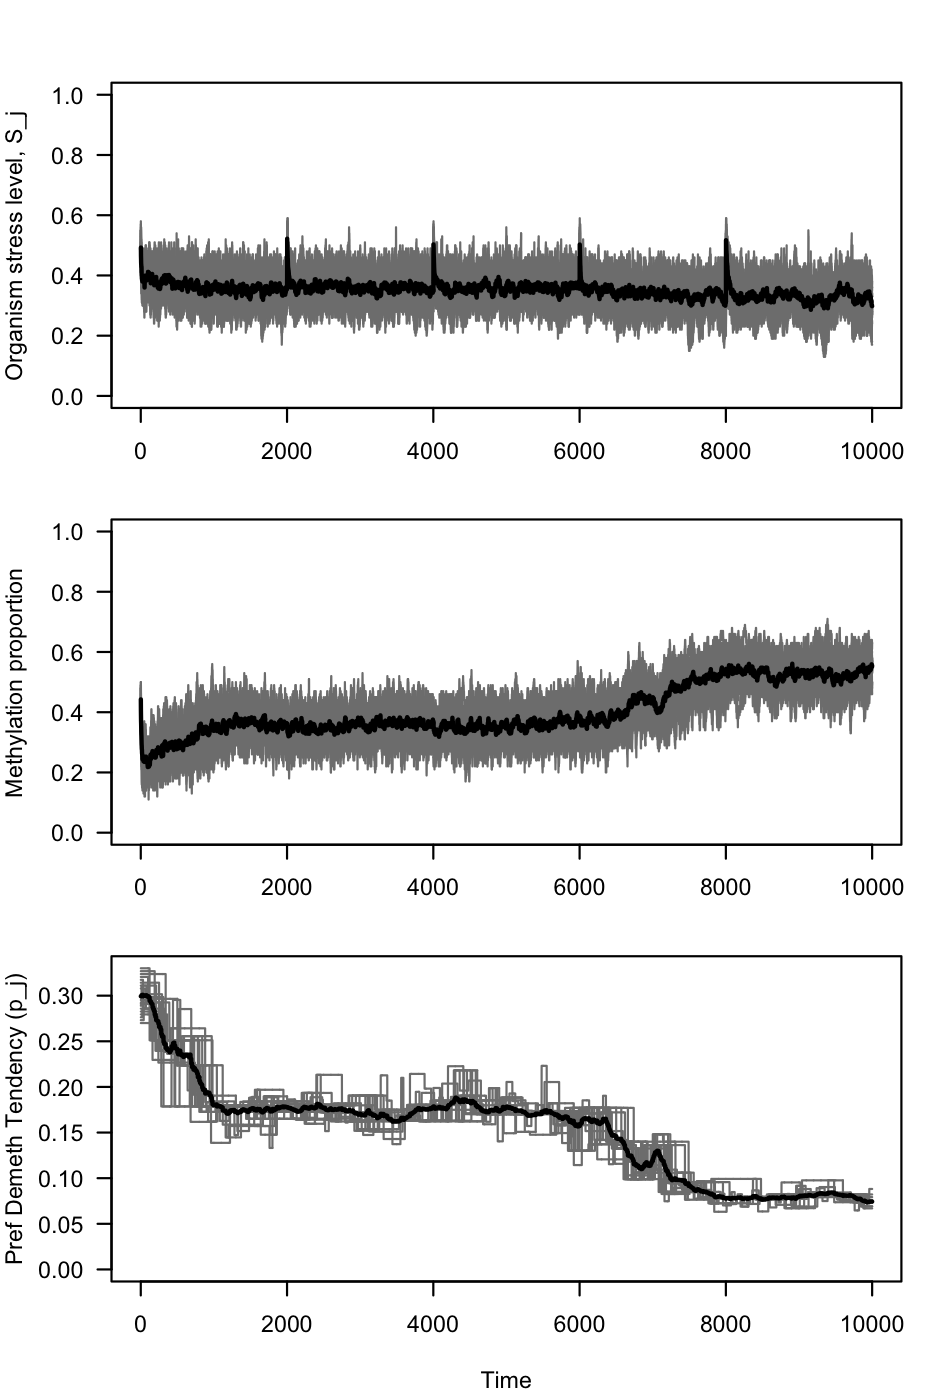
\includegraphics[width=0.8 \textwidth]{Figures/SFig_EvolutionSims.png}
    \caption{\textbf{FOR SUPPLEMENT:} Trajectory of a population with a decreasing marker removal tendency over evolutionary time. The population is subjected to periodic environmental perturbations, which it recovers from, with decreasing stress as beneficial mutations accumulate. These mutations act to reduce the marker removal tendency and thus increase the overall genomic level of epigenetic markers to closer to the environmental mean of 0.5.}
    \label{Sfig:evolutionts}
\end{figure}


\begin{figure}
    \centering
    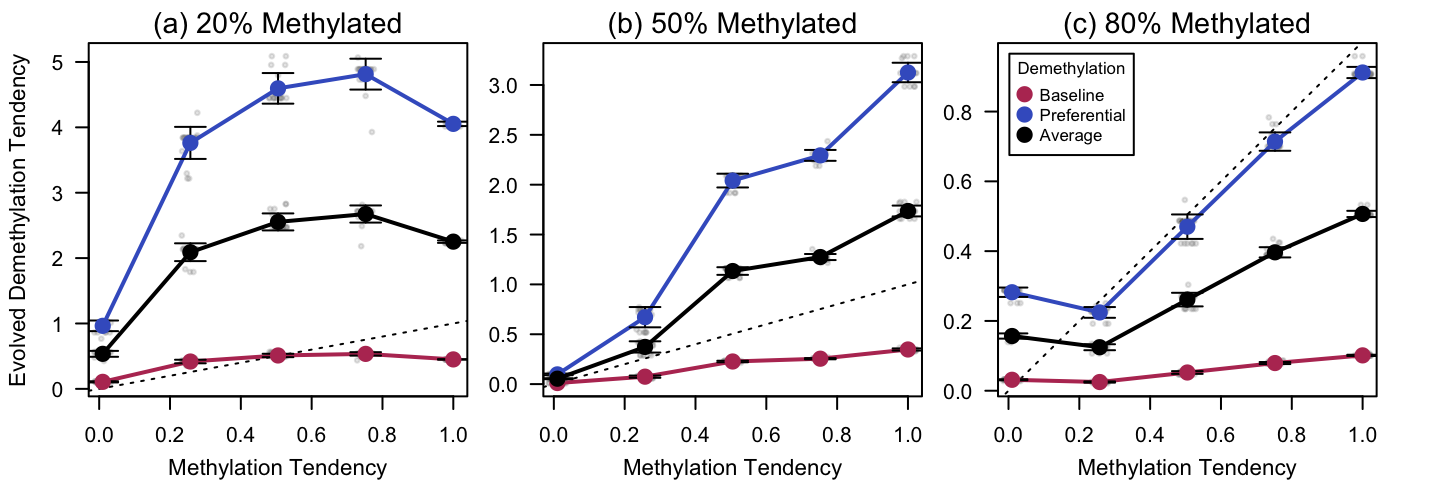
\includegraphics[width= \textwidth]{Figures/Fig_EvolutionSimulation_3cases.png}
    \caption{Evolved stress-minimizing marker removal tendencies as a function of (fixed) addition tendencies. (Note that baseline and preferential marker removal are coupled by $\epsilon = 0.8$.) Generally, as an organism's tendency to add markers in response to stress increases, its tendency to remove markers must increase proportionately. The more markers in the environment that the organism is tracking, the lower the evolved marker removal rates (compare from left to right, noting differences in y-axis scales).}
    \label{Fig:Evolution3panel}
\end{figure}

\begin{figure}
    \centering
    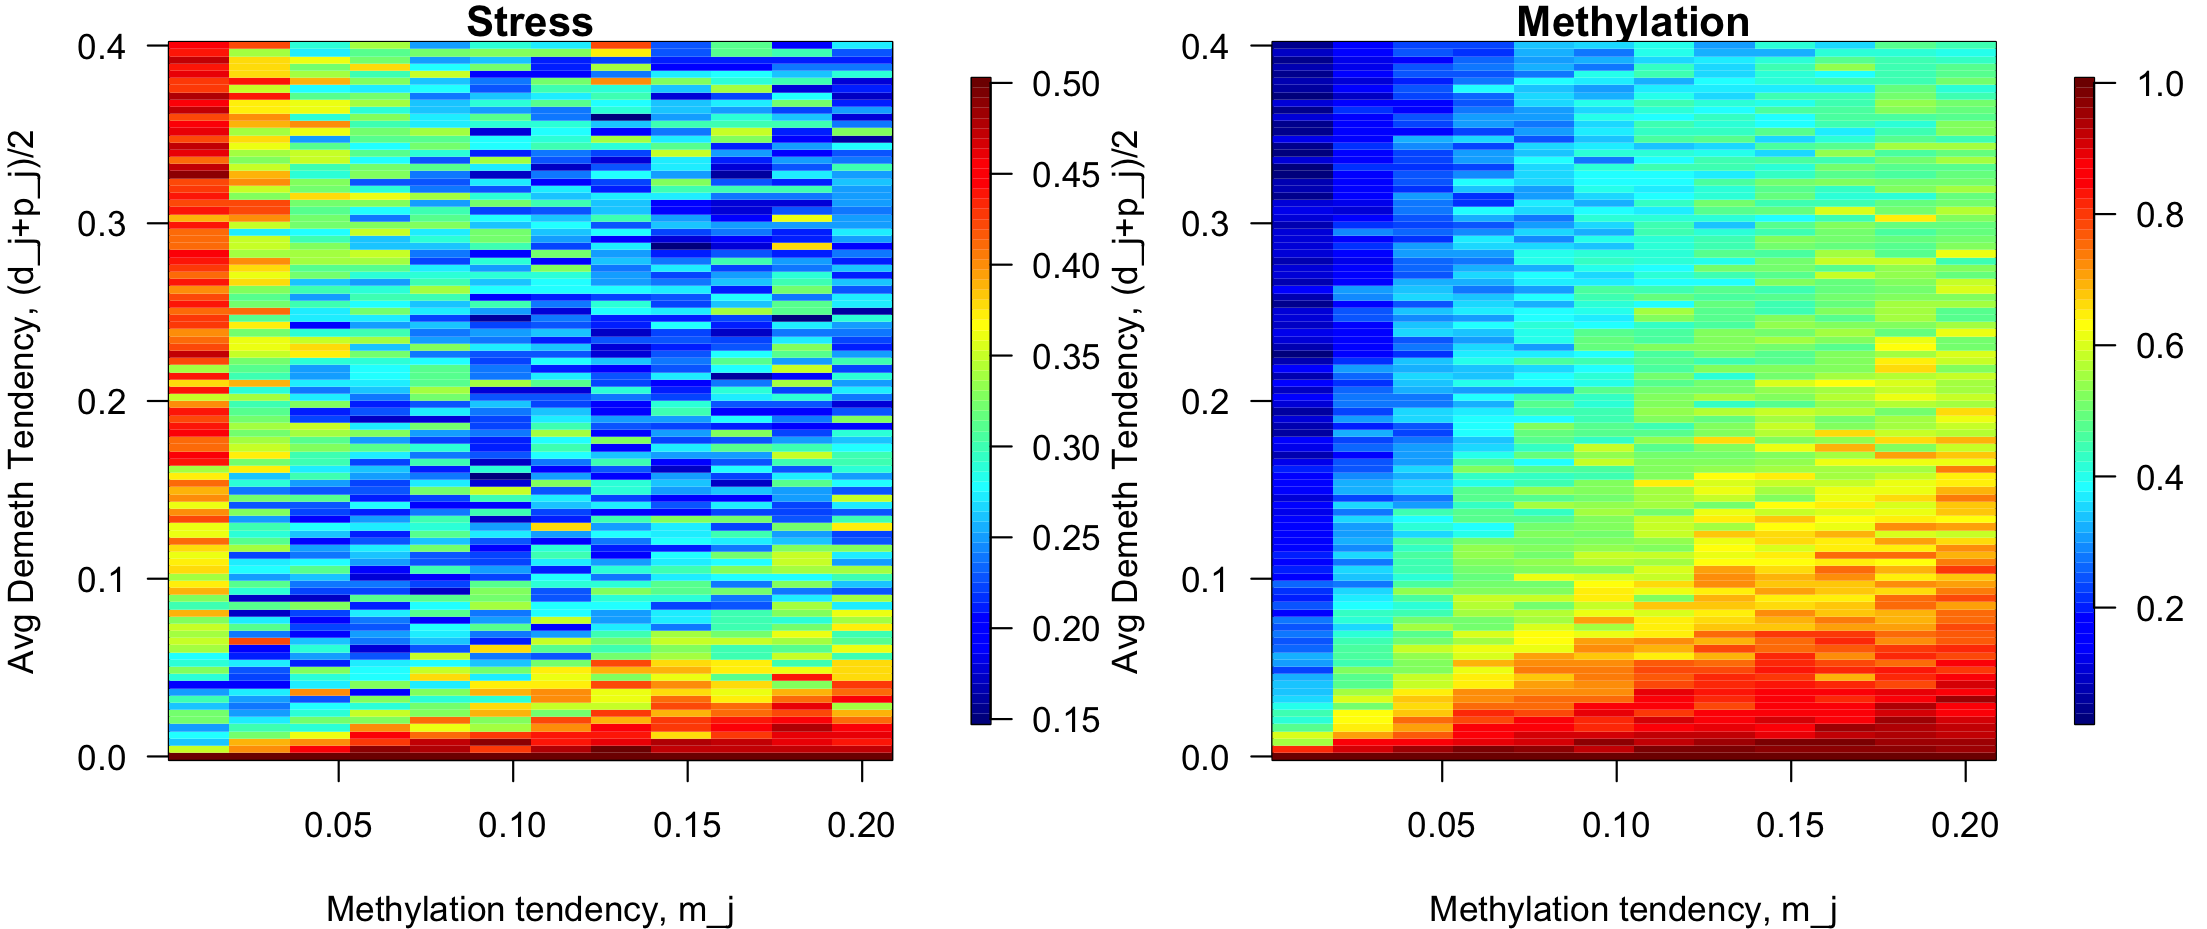
\includegraphics[width= \textwidth]{Figures/Fig_Heatmap_v2.png}
    \caption{\textbf{FOR SUPPLEMENT:} Effects of mismatched epigenetic tendencies on organism performance. If marker removal tendencies are much higher than marker addition tendencies (upper left of both panels), stress is high (left panel) because the organism's number of epigenetic markers is low compared to the environment (right panel). In contrast, relatively low marker removal tendencies lead to high amounts of epigenetic markers on the genome and also high stress (lower right of panels).  }
    \label{SFig:StressHeatmap}
\end{figure}


\subsubsection{Correlational: Organisms appear to maintain homeostasis in epigenetic markers over long timescales.}

Consistent with our model's prediction that organisms should re-equilibrate at a consistent level of epigenetic markers following environmental change (Figure \ref{fig:envfeedback}AB, Figure \ref{fig:methylmismatch}), observational data from SPECIESSSSSS suggest that the amount of epigenetic markers is roughly constant over multiple generations (CITATIONS), and within generations in response to environmental change (CITATIONS). (As discussed above, transient reductions in epigenetic markers in response to environmental perturbations are also consistent with our model's predictions; CITATIONS).



\subsubsection{Mechanism: What mechanisms ensure coupling of addition and removal of epigenetic markers?}

In order to return to and maintain a consistent level of epigenetic markers, organisms must balance the addition and removal of these markers. Our model proposes one, stress-mediated feedback that organisms could use to coordinate epigenetic modifications, but the exact mechanism by which this coordination takes place remains unclear. It is known that the addition and removal of markers are catalyzed by distinct pools of enzymes: for example, ABC and XYZ regulate the addition and removal of histone modification tags respectively (CITATION), and a series of methyl transferase and ABCDEF enzymes regulate the cyclic addition and removal of methyl groupse from cytosines (CITATION). Therefore, organisms may be able to shift their overall levels of epigenetic markers by altering the relative ratios of enzyme and substrate pools [[HOLLIE TO FILL IN MORE DETAILS]].

Epigenetic modification is an energy-requiring process, both for the production of the enzymes necessary to catalyze these reactions and for the high-energy substrates that are needed for the addition and removal of some markers (CITATIONs). Thus, one hypothetical way that epigenetic modification may be linked to environmental stress is through an organism's energetic state. Organisms may only be willing to invest energy in modifying their epigenetic state if they perceive a costly (in terms of energy gain and/or fitness) mismatch with their environment. This also implies (we hypothesize) that organisms that are in a higher energy state (e.g., due to stochastic processes related to resource acquisition, or because they are better able to track their environment quickly) may be best able to track a changing environment. TO understand how rates of epigenet marker addition and removal are coupled to oen another, future studies should examine the quantities of enzymes and substrates, and their activity, over time during an environmental change event and its aftermath.

%Energy and enzymes are required to add \& remove markers, so these processes may be coupled by energetic state of the cell **Energy linkage = important idea to finish on

%KNOWLEDGE GAP: HOW are epigenetic tendencies coupled to one another?




\clearpage

\subsection{Tracking is only effective in certain environments}

Although epigenetic modifications can, in principle, allow organisms to become locally adapted to their environment, epigenetic change must occur on a similar timescale to environmental change to be effective.


\subsubsection{Model Results}

We used our model to explore the relationship between the frequency and magnitude of environmental change and organism stress. To do this, we first implemented a new algorithm for environmental change that allowed the environment to change with predictable fluctuations. Specifically, we simulated a ``band'' of optimally methylated environmental sites that shifted in genome location with a fixed frequency (per number of simulation timesteps) and magnitude (number of genome sites). Examples of how this model can be tuned from periodic, large changes to more frequent, small changes can be seen in Figure \ref{fig:envirovar}.

When environments change relatively rarely (e.g., once every 200 timesteps; Scenario 1 in Figure \ref{fig:envirovar}), organisms with high-information tracking strategies are able to shift their epigenetic state alongside environmental change, minimizing stress even if the environmental change is large in magnitude. However, frequent environmental changes can only be tracked if they are small in magnitude (e.g., Scenario 2 and upper right corner of Figure \ref{fig:envirovar}), and otherwise produce high levels of stress that are comparable to a random epigenetic strategy (expected mean stress of $0.5$).

Our model does not consider any costs for epigenetic modifications, so an organism that attempts to track its environment cannot incur any fitness costs in excess of its mismatch. Thus, our model cannot be used to demonstrate tradeoffs between epigenetic tracking and energy conservation, and does not have selection pressure to reduce epigenetic modification. Incorporating such costs would, however, reveal ``optimal'' epigenetic modification strategies, including abandoning epigenetic change when environmental tracking benefits are less than energetic costs.


The faster the environment shifts, the more (accurate) epigenetic changes must be made to track it. Thus, only organisms with sufficiently high tendencies to add or remove epigenetic markers will be capable of tracking.


\subsubsection{Correlational Knowledge Gap: Do organisms from more variable environments rely more on epigenetic modifications?}

Our model leads to the hypothesis that epigenetic regulation of gene expression is a more effective tool in some environments than others (Figure \ref{fig:envirovar}). Direct tests of this hypothesis are challenging because organisms from different environments are typically also separated by evolutionary history with potential stochastic impacts on epigenetic strategies. However, comparative studies, in which closely related organisms from environments with different degrees of variability, could be used to test this hypothesis... [[STEVEN TO FILL IN FROM HERE]]

\subsubsection{Mechanistic Knowledge Gap: What granularity of environmental change can organisms sense?}

A corollary to our above hypothesis is that organisms should evolve epigenetically mediated responses to environmental conditions that (1) recur frequently enough that the benefits of an epigenetic response outweigh their costs (and therefore the epigenetic response is evolutionarily maintained), and (2) are best addressed through reversible modification of gene expression. For example, experiments and models exploring the phenomenon of bet-hedging strategies (phenotypic variation that buffers an organism's fitness in variable environments, CITATION) demonstrate that these strategies should only evolve when the timescales of environmental variation are aligned with the timescales of an organism's life history (Rainey et al CITATION). However, while a growing body of literature demonstrates a capacity for epigenetic remodeling in response to environmental change (CITATIONS), we still do not know the granularity of environmental change that organisms can sense. Given evidence for both within-generation epigenetic modification (CITATIONS) and trans-generational epigenetic inheritance (CITATIONS), we posit environmental changes that occur once every two or fewer generations, but persist for at least one reproductive cycle, are those most likely to produce an evolved epigenetic response. However, these environmental change should be cyclic or at least reversible, thus selecting for transient epigenetic modifications of gene expression, as opposed to permanent, directional evolutionary change. 

By better understanding the frequency, speed, and environmental sensitivity of epigenetic modification experimentally and observationally, we can therefore make hypotheses about the types of environmental variation that lineages experienced over evolutionary time. 



\subsubsection{Knowledge Gap}

\textit{Comparative studies of organisms in low vs high fluctuating environments, to ask which ones have epigenetic tracking modifications?}

\begin{figure}
    \centering
    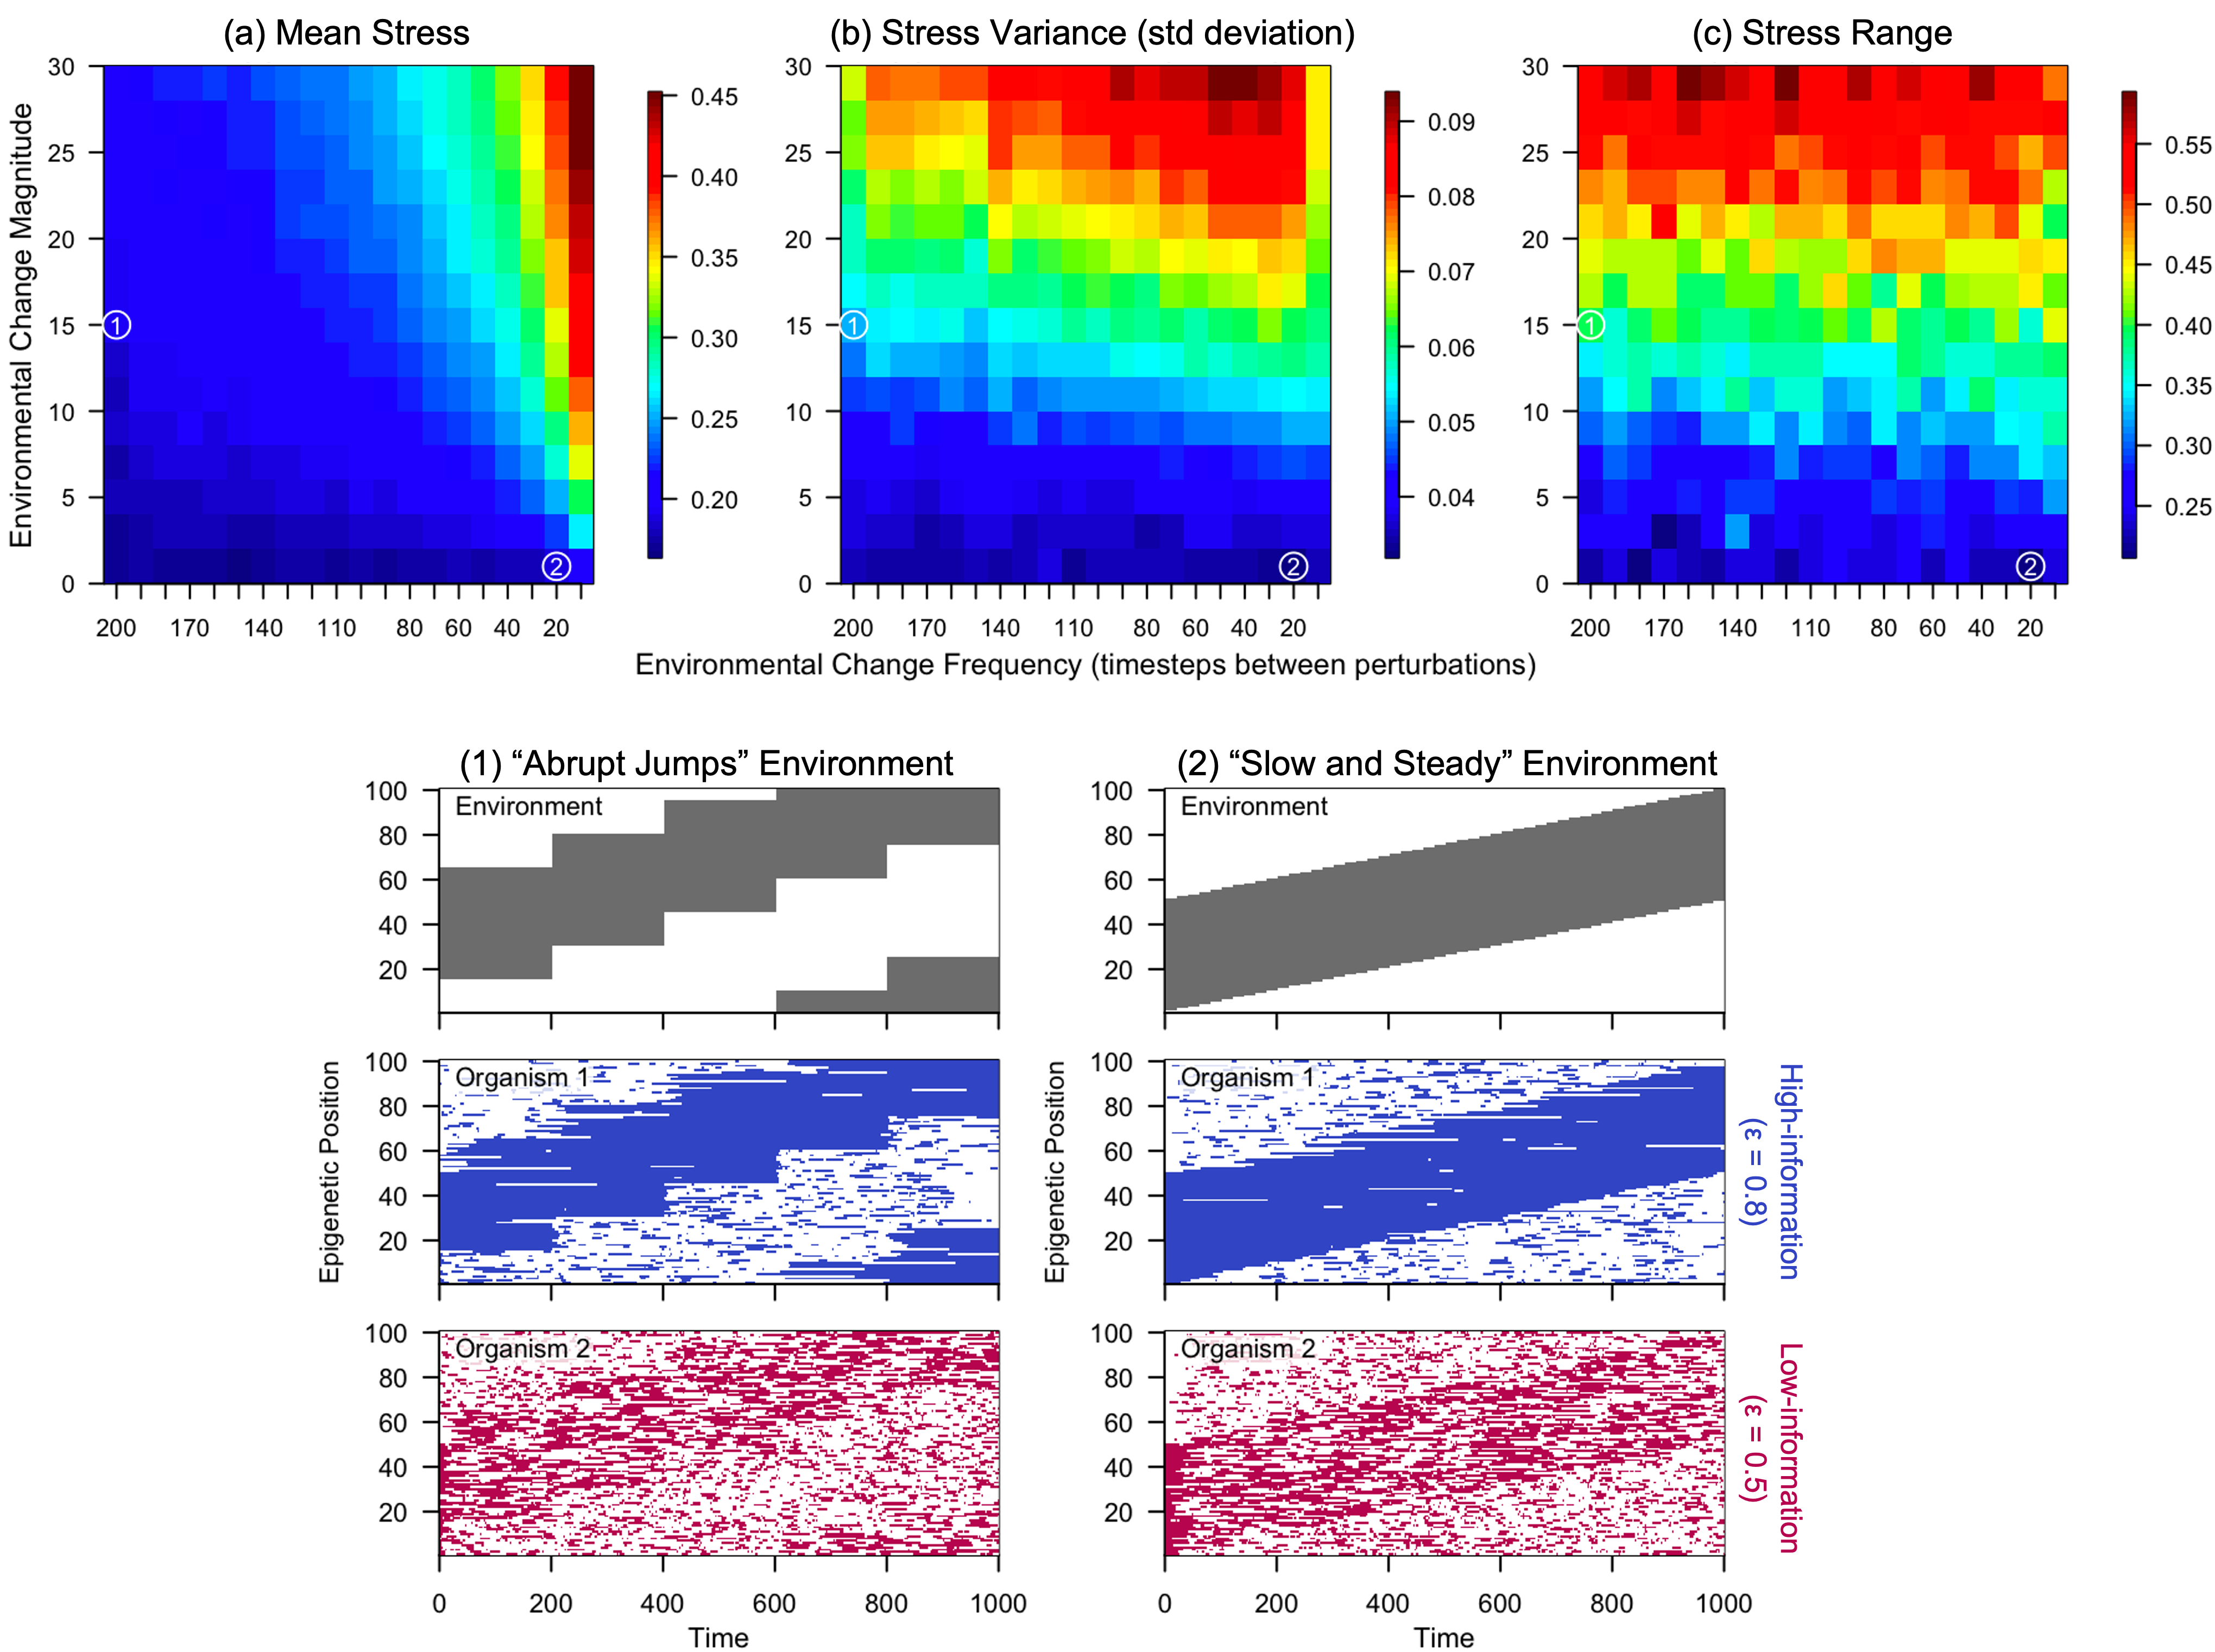
\includegraphics[width=\textwidth]{Figures/Fig_EnvironmentalSimulationComposite.png}
    \caption{\textbf{Effects of environmental change on organism performance.} (a) An organism with strong environmental tracking ($\epsilon = 0.99$) is able to track environments that change with low frequency or low magnitude. (b) However, high-magnitude changes result in large variance in stress levels, because of transient periods of re-equilibration to environmental conditions immediately following a shift in the environmental state. When changes are frequent and high-variance, stress variance actually decreases because of the extremely poor match to the environment. (c) Overall, larger magnitude shifts produce greater range in stress (comparing minimum to maximum values over the course of the simulation) because of periodic spikes in stress level. Below: Example scenarios (also marked on the heatmaps) for (1) low-frequency, intermediate-amplitude, and (2) high-frequency, low-amplitude environmental change. Filled area indicates a site with an epigenetic marker in the environment (top row, gray), an organism with a high degree of tracking (middle row, blue), and an organism with a low degree of tracking (bottom row, pink). Organisms with high levels of environmental information ($\epsilon = 0.99$) track better, especially in environments with larger magnitudes of change.}
    \label{fig:envirovar}
\end{figure}


\clearpage


\bibliography{bibliography}



% \clearpage

% \ 

% \clearpage

% \ 

% \clearpage

% \section{OLD TEXT/FIGURES:}

% \subsection{Coupling epigenetic rates}
% \textbf{This section will be deleted later.} One limitation of this model is that there is an ``obvious'' optimal solution: An organism that wishes to minimize its stress should simultaneously (1) minimize its probability of random demethylation (i.e., set $d_j = 0$), and (2) maximize its probability of preferential methylation (i.e., set $p_j$ very large). 

% This is in contrast to the ``original'' formulation of the model, in which stress drove epigenetic change in a fixed number of sites. (More stress = more sites changed.) In this case, if you ``ran out'' of sites to preferentially change, you would start changing non-preferred (i.e., incorrect) sites. So there was a ``natural coupling'' between tendencies for methylation and demethylation.

% There's some biology to think about here. Perhaps stress results in the production of enzymes that can catalyze epigenetic modification. These enzymes might be ``looking for something to do.'' Thus producing lots of these enzymes (having a high tendency) might result in more ``errors'' if all the preferential sites are already modified. This means that $d_j$ and $p_j$ might be coupled in some way.

% One way to do this is by assuming that $d_j$ and $p_j$ are related to one another, and to $m_j$, an individual's tendency for methylation.

% \subsubsection{OPTION 1: MEAN DEMETHYLATION IS PROPORTIONAL TO METHYLATION}

% We might assume that $d_j$ is some deviation $\epsilon$ less than $m_j$, and $p_j$ is the same deviation away in the opposite direction:

% \begin{equation}
%     m_j = \frac{\left( d_j - \epsilon \right) + \left( p_j + \epsilon \right)}{2}
% \end{equation}

% If we want the baseline rates of methylation and demethylation to differ, we can introduce the baseline multiplier $b$, which can take on values greater or less than 1 to represent greater or smaller tendencies to demethylate, respectively.

% \begin{equation}
%     m_j = \frac{b\left[ \left( d_j - \epsilon \right) + \left( p_j + \epsilon \right) \right]}{2}
% \end{equation}

% Similarly, we can treat $\epsilon$ as a proportional perturbation, e.g.:

% \begin{equation}
%     m_j = \frac{b\left[ d_j\left( 1 - \epsilon \right) + p_j \left( 1+ \epsilon \right) \right]}{2}
% \end{equation}
% Here, we choose $0 \leq \epsilon \leq 1$ so that all demethylation probabilities are nonnegative. \textbf{This is the version used in the current incarnation of the model.}

% \subsubsection{OPTION 2: PREFERENTIAL AND RANDOM DEMETHYLATION HAVE A FIXED COUPLING}

% We could also assume that $p_j$ and $d_j$ are related to one another in a fixed way. They could have a fixed difference, e.g.:
% \begin{equation}
%     p_j = d_j + \epsilon,
% \end{equation}
% or be proportional, e.g.:
% \begin{equation}
%     p_j = \epsilon d_j.
% \end{equation}

% \subsubsection{OTHER OPTIONS?}
% All suggestions accepted.

% \section{More on environmental tracking...}
% We demonstrated this phenomenon in our mathematical model by showing how different epigenetic tendencies intersected with the frequency of environmental change. 

% \textit{For now, I have a couple placeholder timeseries figures  (Figures \ref{fig:changerates}-\ref{fig:changerates2}), but I plan to make something more sophisticated in future.}

% \textit{One thing to think about here is that the higher your epigenetic tendencies are, the faster you're going to get to the stress minimum. Is there a natural ``upper bound'' on these tendencies? Like if you make them large, you have more variance in the population? Preliminary analyses (Figure \ref{fig:methyltendency}) didn't support this. Maybe if your rates are too fast, evolution doesn't work as well because there's more of a chance someone with a ``poor'' tendency just stochastically has the highest fitness?}

% \begin{figure}
%     \centering
%     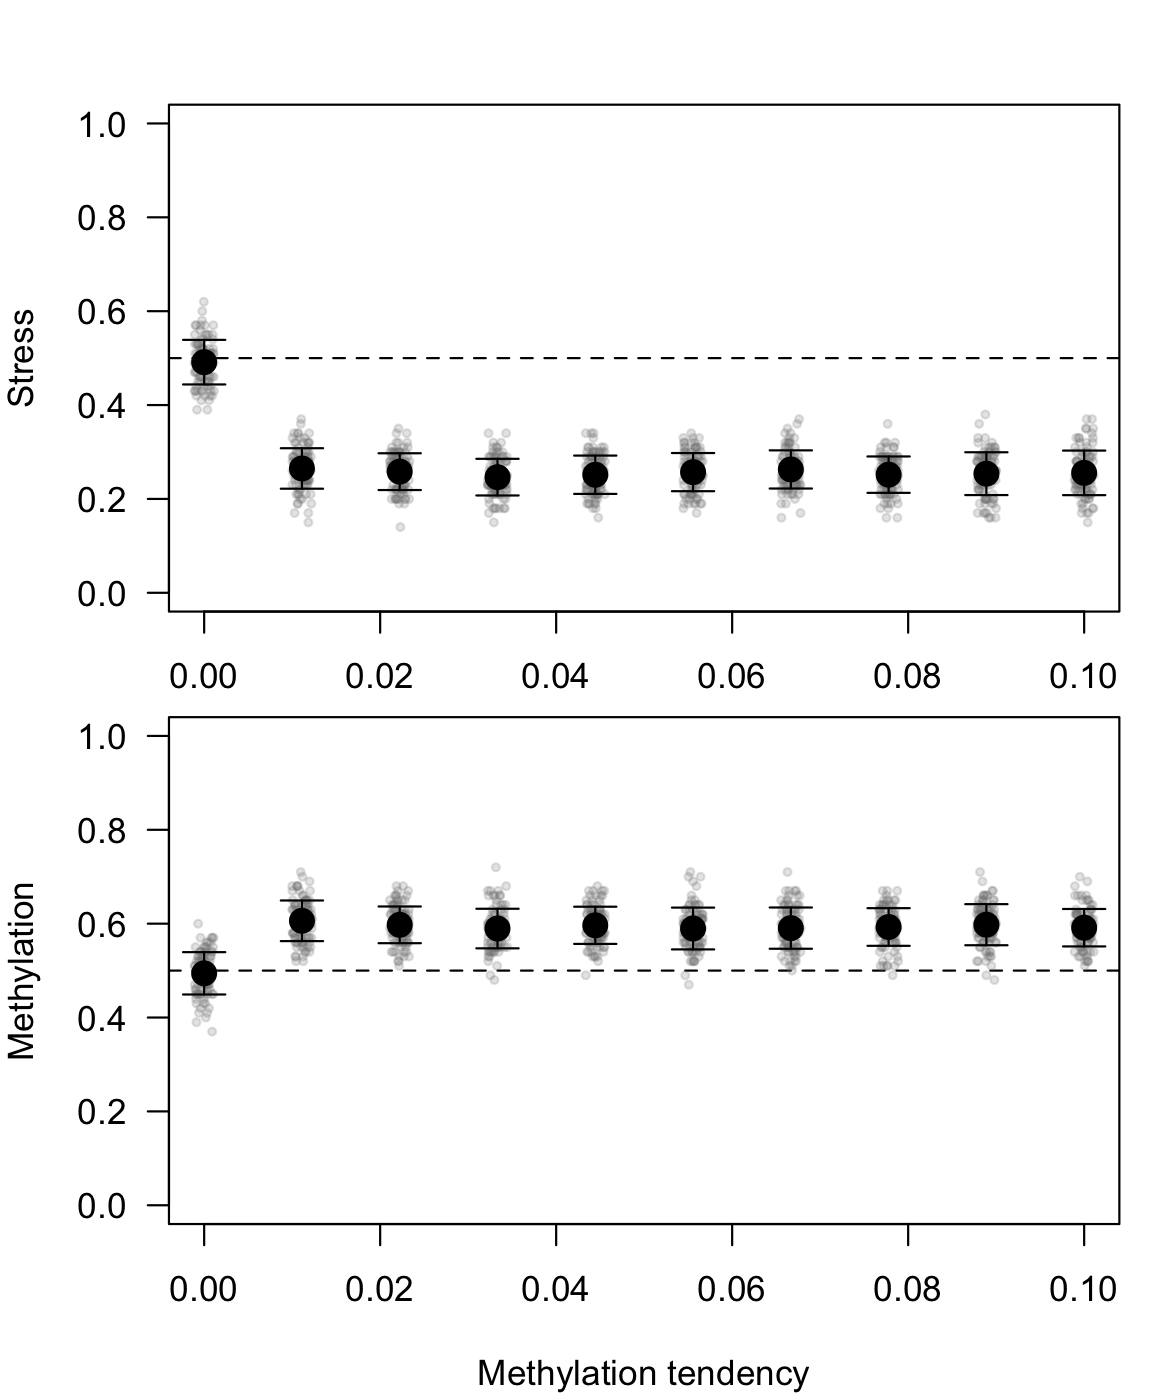
\includegraphics[width=0.8 \textwidth]{Figures/SFig_MethylationTendency.png}
%     \caption{Methylation tendency affects the rate of approach (not shown) but not the eventual stress levels or methylation rates that an organism experiences. Epsilon 0.8. Base multiplier 1. \textbf{This is for the supplement.}}
%     \label{fig:methyltendency}
% \end{figure}

% \begin{figure}
%     \centering
%     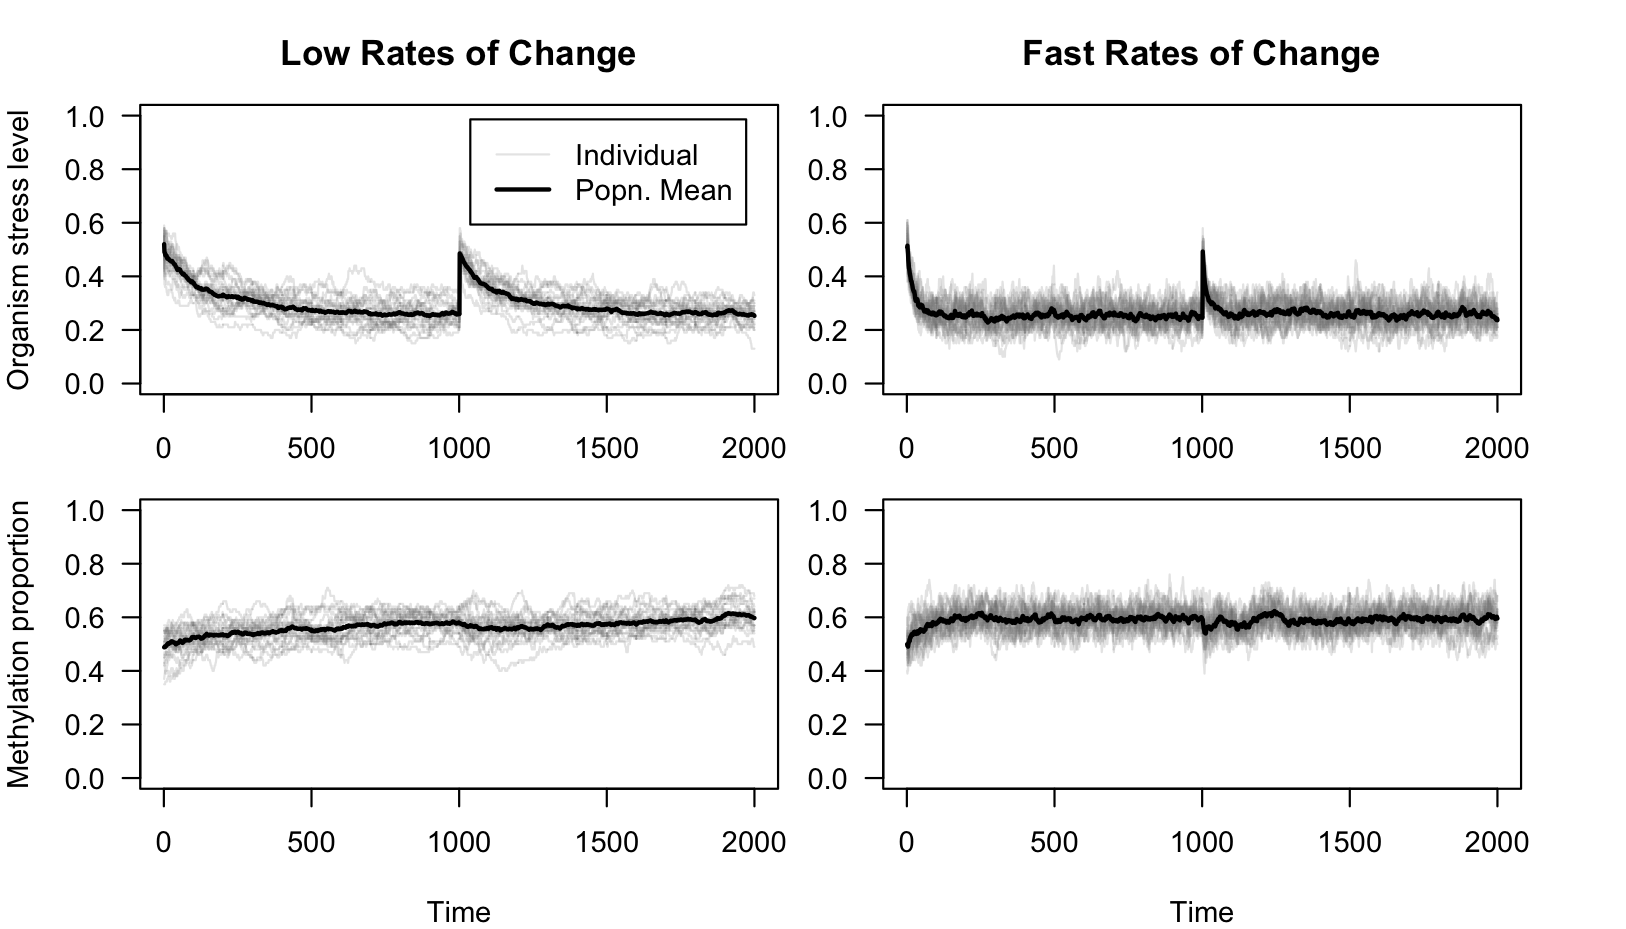
\includegraphics[width= 0.9 \textwidth]{Figures/Fig_ChangeRates.png}
%     \caption{Contrast in the time to minimum stress for two different epigenetic tendencies. Baseline methylation tendency of 0.01 (left; slow) and 0.1 (right; fast). Epsilon 0.8. Base multiplier 1.}
%     \label{fig:changerates}
% \end{figure}

% \begin{figure}
%     \centering
%     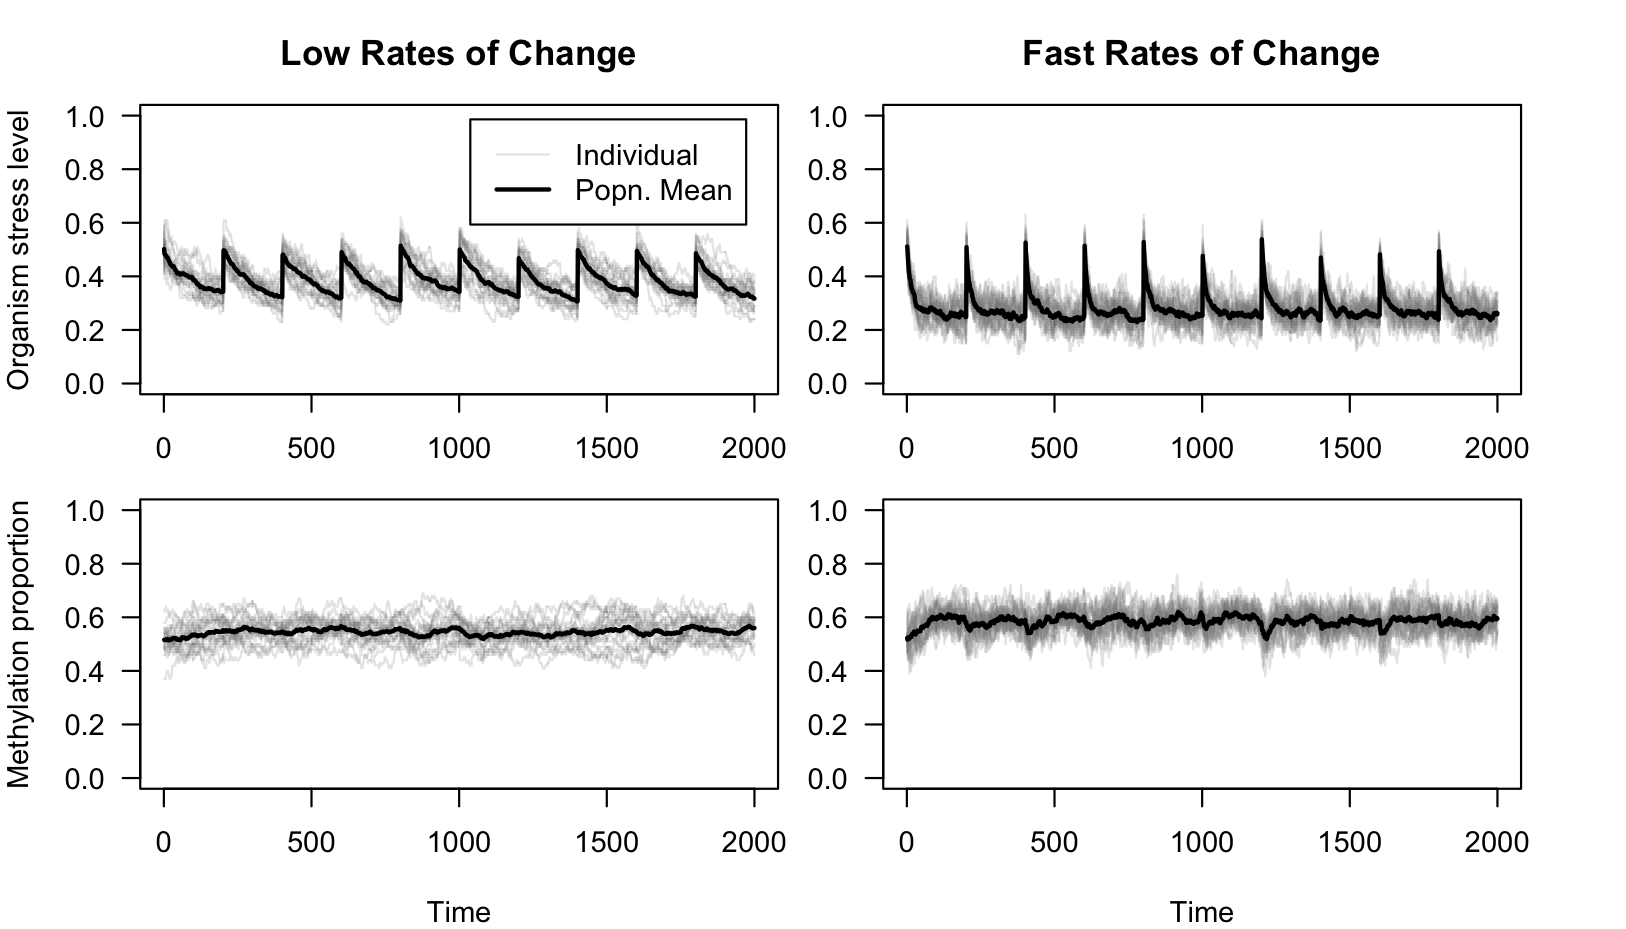
\includegraphics[width= 0.9 \textwidth]{Figures/Fig_ChangeRates_freqshifts.png}
%     \caption{Same organismal biology as Figure \ref{fig:changerates}, but with more frequent environmental change. Note that in this case, the organisms with relatively slow epigenetic change don't achieve low stress before the environment changes again. Baseline methylation tendency of 0.01 (left) and 0.1 (right). Epsilon 0.8. Base multiplier 1.}
%     \label{fig:changerates2}
% \end{figure}

% \subsubsection{Empirical Data}
% \subsubsection{Knowledge Gap}

\end{document}
